\documentclass{article}
\usepackage{xeCJK}
\usepackage{tikz}
\usepackage{amsmath}
\usepackage{fontspec}
\usepackage{zhnumber}
\renewcommand\thesection{\zhnum{section}}
\renewcommand\thesubsection{\arabic{subsection}}
\setmainfont{Times New Roman} % 設置主要的英文字體
\setCJKmainfont{微軟正黑體} % 設置主要的中文字體
\title{線性代數初探}
\author{連廷恩\\
    1628,\ 國立臺灣師範大學附屬高級中學}
\date{2025年1月}

\begin{document}

    \begin{titlepage}
        \maketitle
        \vspace{2cm}
    \end{titlepage}

    \centerline{\huge{摘要}}\vspace{2cm}\par
        由於對向量空間的興趣與對電腦科學的憧憬,我將在本文嘗試學習線性代數。\\
        我嘗試搭配MIT在Youtube上的公開課程"MIT 18.06 Linear Algebra"來學習一些線性代數的知識,並且在本文中以自己的方式紀錄知識。\\
        本文將以\LaTeX 進行撰寫,並且上傳至GitHub以記錄版本更新。\\
        在本文之程式碼中,您也能看見本人對\LaTeX 的學習進度。\\

    \tableofcontents
    \newpage
    \section{甚麼是線性代數?}
    \newpage
    \section{圖像化的線性方程組}
    \subsection{列:方程式交點}
        \par
        在列看法中,方程組將直觀地被轉換成一個比線性空間維度低一維的「平面」。例如二維平面上的一組方程組,其解便是平面上兩直線的一個交點。\\
        讓我們先用一個二元一次方程組來解釋。\\

        \begin{equation}
            \left\{
                \begin{array}{c}
                    2x + 3y = 6\\
                    4x + 5y = 10
                \end{array}
            \right.
        \end{equation}

        \par
        這是一個簡單的二元一次方程組,我們甚至能用瞪眼法看出 x = 0, y = 2 是這個線性方程組的解。\\
        但這個方程組可以寫成矩陣的形式,就像這樣。\vspace{0.5cm}\\
        \centerline{
        $\begin{bmatrix}
            2&3\\
            4&5
        \end{bmatrix}$
        $\times $
        $\begin{bmatrix}
            x\\
            y
        \end{bmatrix}$
        $=$
        $\begin{bmatrix}
            6\\
            10
        \end{bmatrix}$
        }
        \\
        \centerline{
            A $\times$ x = b
        }\vspace{0.5cm}
        
        \par
        若是繪製函數圖形,我們可以獲得下圖。\\

        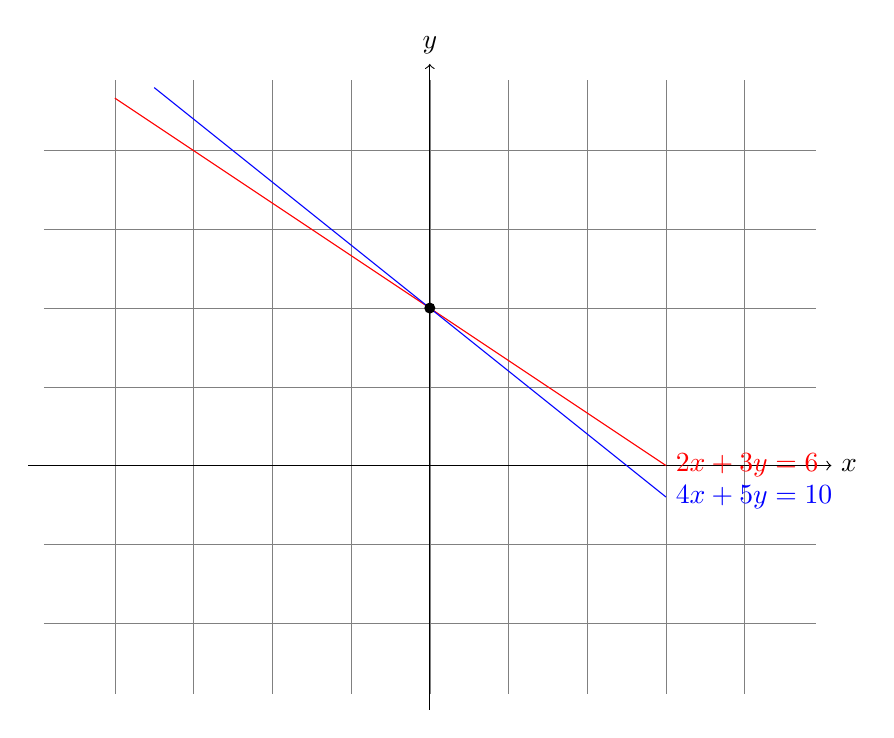
\begin{tikzpicture}
            \draw[color=gray,very thin] (-4.9,-2.9) grid (4.9,4.9);
            \draw[->] (-5.1,0) -- (5.1,0) node[right] {$x$};
            \draw[->] (0,-3.1) -- (0,5.1) node[above] {$y$};
            \draw[color=red,domain=-4:3] plot({\x},{-2/3*\x+2}) node[right] {$2x + 3y = 6$};
            \draw[color=blue,domain=-3.5:3] plot({\x},{-4/5*\x+2}) node[right] {$4x + 5y = 10$};
            \fill (0,2) circle(2pt);
        \end{tikzpicture}

    \subsection{行:向量組合}
        \par
        用上一個例子,我們可以將方程組寫成線性組合的形式:兩個伸縮了分別x倍與y倍的向量組合成一個新向量。\vspace{0.5cm}\\
        \centerline{
            $\mathcal{X}$
            $\begin{bmatrix}
                2\\
                4
            \end{bmatrix}$
            $+$
            $\mathcal{Y}$
            $\begin{bmatrix}
                3\\
                5
                \end{bmatrix}$
            $=$
            $\begin{bmatrix}
                6\\
                10
                \end{bmatrix}$
        }\\
        \centerline{
            $\vec{A}$X$+$ $\vec{B}$Y$=$ $\vec{C}$
        }
        同樣的,我們將這行線性組合繪製在二維平面上來取得圖像化的成果。\\
        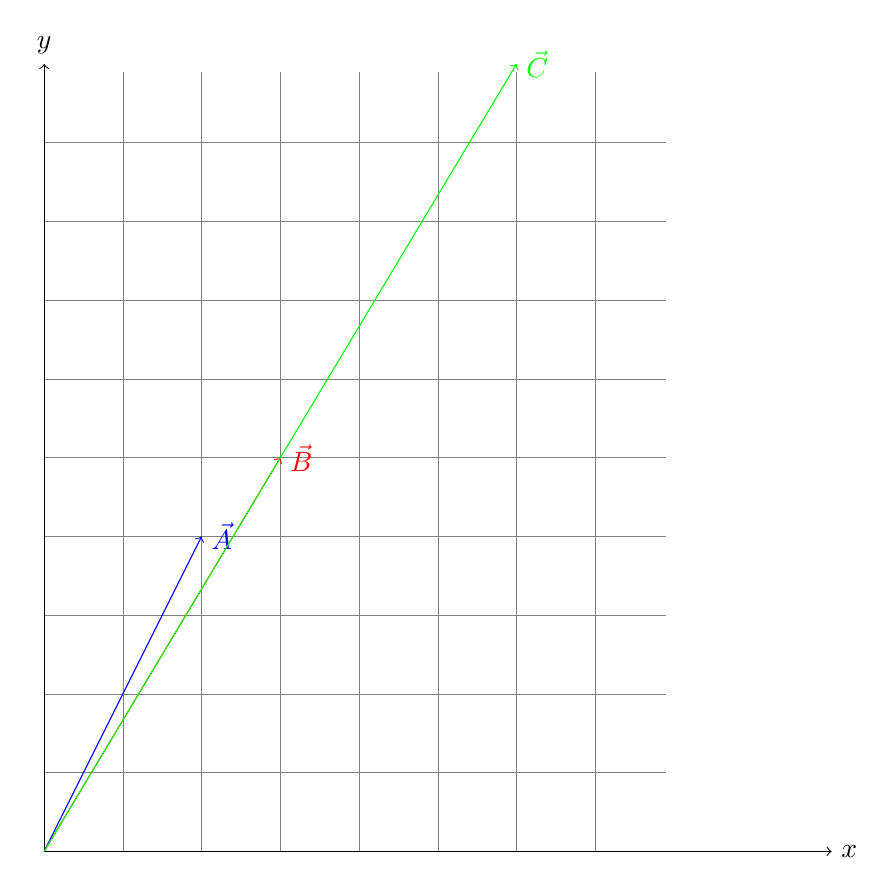
\begin{tikzpicture}
            \draw[color=gray,very thin] (0,0) grid (7.9,9.9);
            \draw[->] (0,0) -- (10,0) node[right] {$x$};
            \draw[->] (0,0) -- (0,10) node[above] {$y$};
            \draw[->,color=blue] (0,0) -- (2,4) node[right] {$\vec{A} $};
            \draw[->,color=red] (0,0) -- (3,5) node[right] {$\vec{B} $};
            \draw[->,color=green] (0,0) -- (6,10) node[right] {$\vec{C} $};
        \end{tikzpicture}\vspace{1cm}
        \par
        可以看得出來,$\vec{C}$就是$\vec{B}$伸長兩倍後得到的向量,由此可知x = 0,y = 2是這個線性方程組的解。\\
%1/25 process.
\end{document}
